\documentclass[11pt]{beamer}    % Presentacion
\usepackage[spanish]{babel}     % Español
\usepackage[utf8]{inputenc}     % Aceptar entrada UTF-8
\usepackage{graphicx}           % Insertar imagenes
\usepackage{float}              % Entornos flotantes
\usepackage{pgfgantt}           % Diagrama de Gantt
\usepackage{subcaption}


\usetheme{metropolis}           % Usar el tema metropolis
\setlength{\unitlength}{1cm}    % Configurar el entorno picture
%%%%%%%%%%%%%%%%%%%%%%%%%%%%%%%%%%%%%%%%%%%%%%%%%%%%%%%%%%%%%%%%%%%%%%%%%%%%%%%%
% Configurar footer
%\setbeamertemplate{frame footer}{\insertshortauthor \quad \quad \insertshortsubtitle}
%\setbeamercolor{footline}{fg=gray}
\setbeamertemplate{section in toc}[sections numbered]
\metroset{numbering=fraction}
%%%%%%%%%%%%%%%%%%%%%%%%%%%%%%%%%%%%%%%%%%%%%%%%%%%%%%%%%%%%%%%%%%%%%%%%%%%%%%%%
% Portada
\title{Desarrollo de una arquitectura reactiva y deliberativa usando
planificación en el entorno de juegos GVGAI}
\subtitle{Trabajo Fin de Grado}
\author[Vladislav Nikolov]{\textbf{Autor:} Vladislav Nikolov Vasilev \and
    \textbf{Director:} Juan Fernández Olivares
}
\date{\today}
\institute{Departamento de Ciencias de la Computación e Inteligencia Artificial \\
    Escuela Técnica Superior de Ingenierías Informática y de Telecomunicación \\
    Universidad de Granada
}

\begin{document}
    % Insertar pagina de titulo
    \maketitle

    % Insertar indice
    \begin{frame}{Índice}
        \tableofcontents
    \end{frame}

    \section{Introducción}
    \begin{frame}{Motivación}
        \begin{itemize}
            \item Planificación automática como potente herramienta para la resolución de problemas.

            \item Integrada exitosamente en aplicaciones reales pero no en videojuegos.

            \item Videojuegos presentan entornos \alert{dinámicos} y \alert{complejos}.
            No se puede dar una respuesta rápida.

            \item Desarrollo de agentes para juegos concretos cuya componente deliberativa se basa
            en planificación.
        \end{itemize}
    \end{frame}

    \begin{frame}{Objetivo}
        Creación de una arquitectura en el entorno de juegos GVGAI con las siguientes características:

        \begin{enumerate}
            \item Combina componente \alert{reactiva} con \alert{deliberativa} basada en planificación.
            \item Lo suficientemente \textbf{general} para resolver cualquier juego del entorno.
        \end{enumerate}
    \end{frame}

    \begin{frame}{Contribuciones principales}
        \begin{itemize}
            \item Nuevas vías para experimentar con técnicas de planificación en GVGAI.
            \item Herramienta educativa.
        \end{itemize}
    \end{frame}

    %%%%%%%%%%%%%%%%%%%%%%%%%%%%%%%%%%%%%%%%%%%%%%%%%%%%%%%%%%%%%%%%%%%%%%%%%%%%%%%%
    \section{Antecedentes}

    \begin{frame}{Trabajos relacionados}
        Propuesta \alert{novedosa}, aunque se han desarrollado arquitecturas para otros
        juegos en específico.

        \begin{figure}
            \centering
            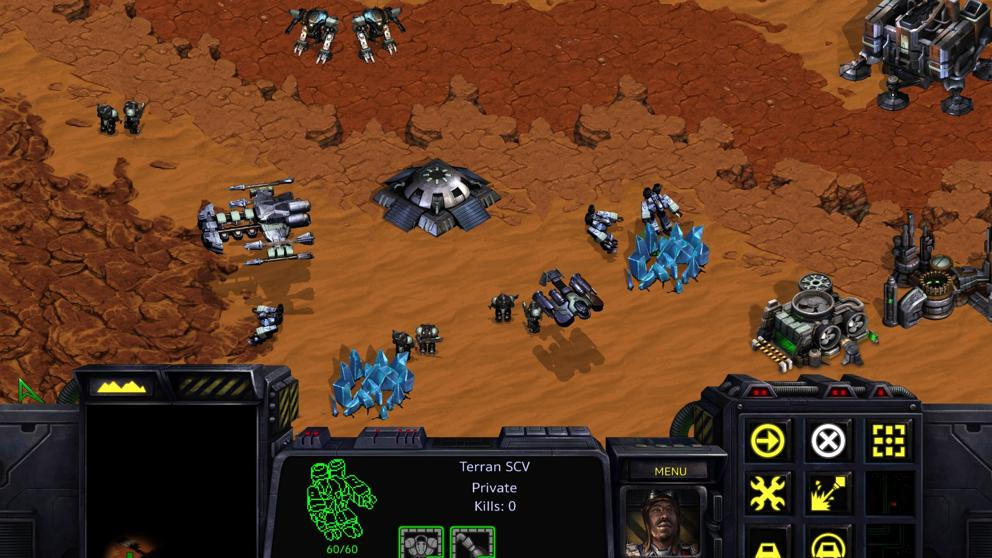
\includegraphics[scale=0.25]{img/presentation/starcraft}
        \end{figure}
    \end{frame}

    \begin{frame}{Planificación}
        \begin{figure}
            \centering
            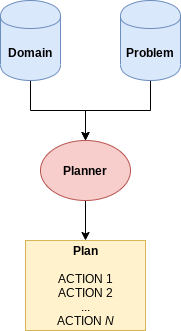
\includegraphics[scale=0.4]{img/presentation/planning}
        \end{figure}
    \end{frame}

    \begin{frame}{PDDL}
        \begin{figure}
            \centering
            \begin{subfigure}[t]{.55\textwidth}
                \centering
                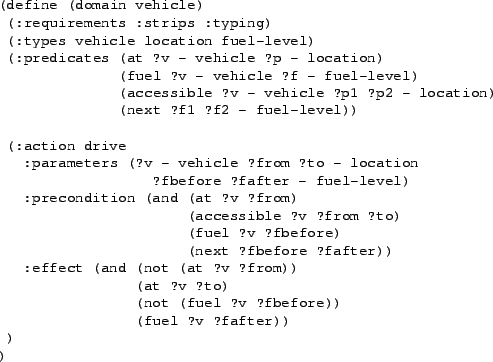
\includegraphics[scale=0.32]{img/presentation/pddl_domain}
                \caption{Dominio de planificación PDDL.}
            \end{subfigure}%
            \begin{subfigure}[t]{.45\textwidth}
                \centering
                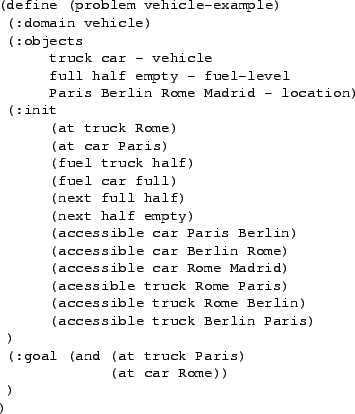
\includegraphics[scale=0.32]{img/presentation/pddl_problem}
                \caption{Problema de planificación PDDL.}
            \end{subfigure}
        \end{figure}
    \end{frame}

    \begin{frame}{Planning.Domains}
        \begin{figure}
            \centering
            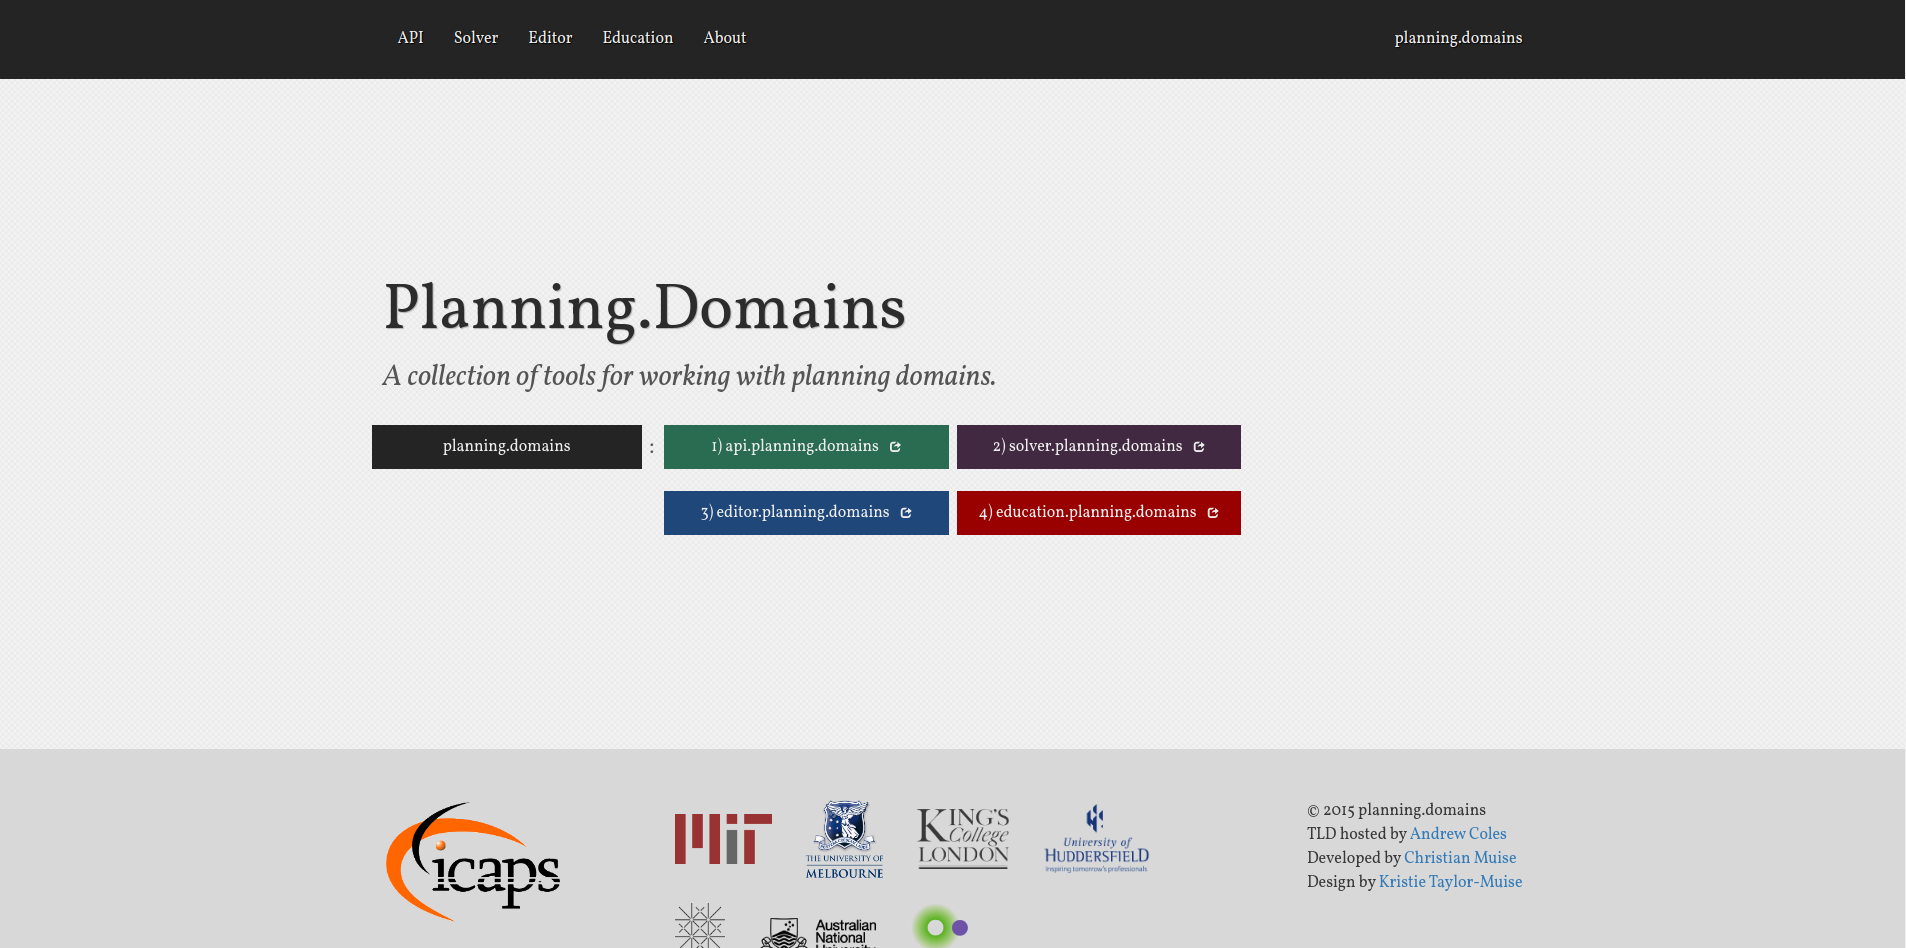
\includegraphics[scale=0.23]{img/presentation/planning-domains}
        \end{figure}
    \end{frame}

    \begin{frame}{GVGAI}
        \begin{figure}
            \centering
            \begin{subfigure}[t]{.5\textwidth}
                \centering
                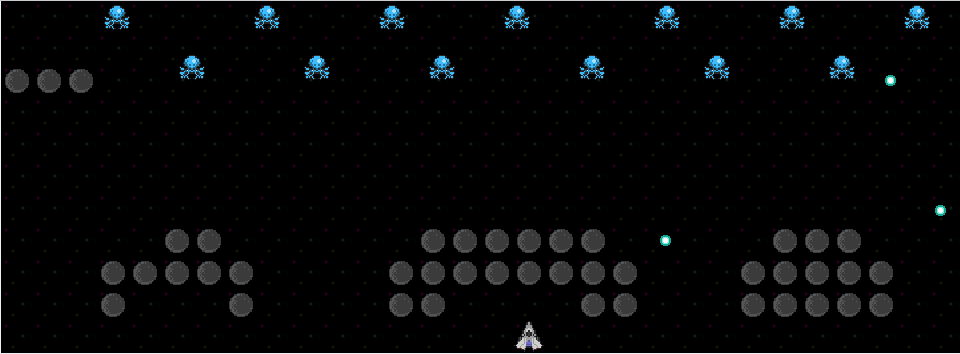
\includegraphics[scale=0.2]{img/presentation/aliens}
            \end{subfigure}%
            \begin{subfigure}[t]{.5\textwidth}
                \centering
                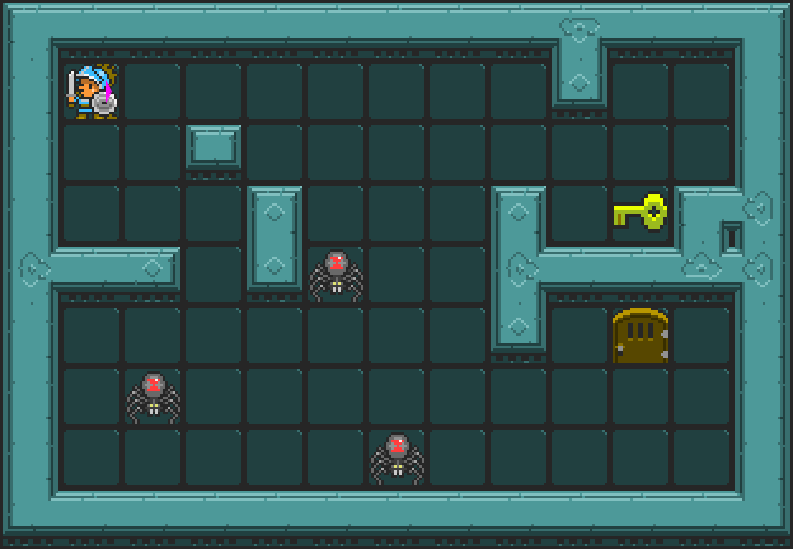
\includegraphics[scale=0.2]{img/presentation/zelda}
            \end{subfigure}
            \par\bigskip
            \begin{subfigure}[t]{.5\textwidth}
                \centering
                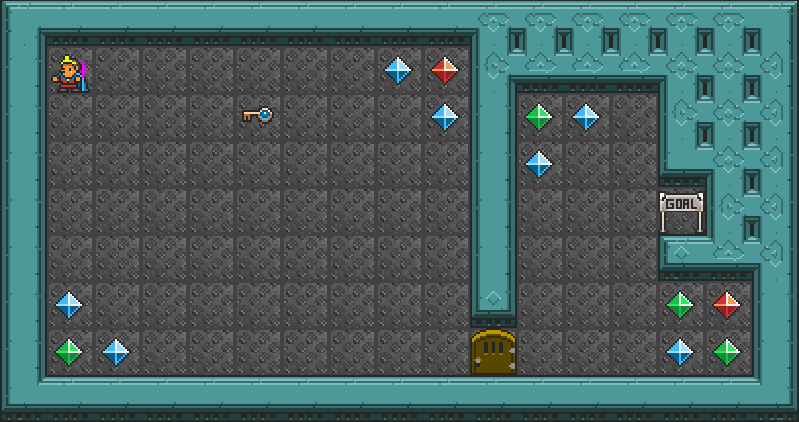
\includegraphics[scale=0.2]{img/presentation/brainman}
            \end{subfigure}%
            \begin{subfigure}[t]{.5\textwidth}
                \centering
                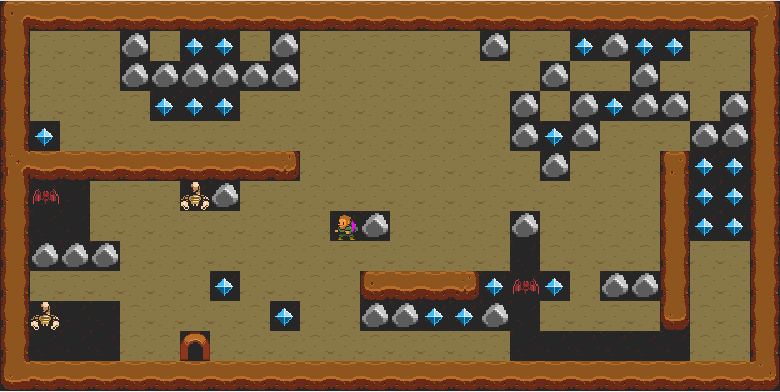
\includegraphics[scale=0.2]{img/presentation/boulderdash}
            \end{subfigure}
        \end{figure}
    \end{frame}

    \begin{frame}{VGDL}
        \begin{figure}
            \centering
            \begin{subfigure}{0.5\textwidth}
                \centering
                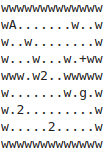
\includegraphics[scale=0.5]{img/presentation/game_lvl}
                \par\bigskip
                {\LARGE$\downarrow{}$}
                \par\bigskip
                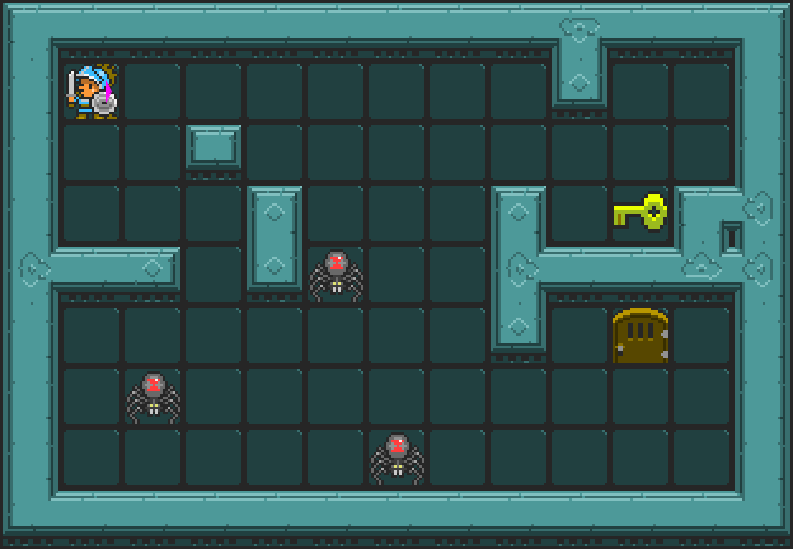
\includegraphics[scale=0.2]{img/presentation/zelda}
            \end{subfigure}%
            \begin{subfigure}{0.5\textwidth}
                \centering
                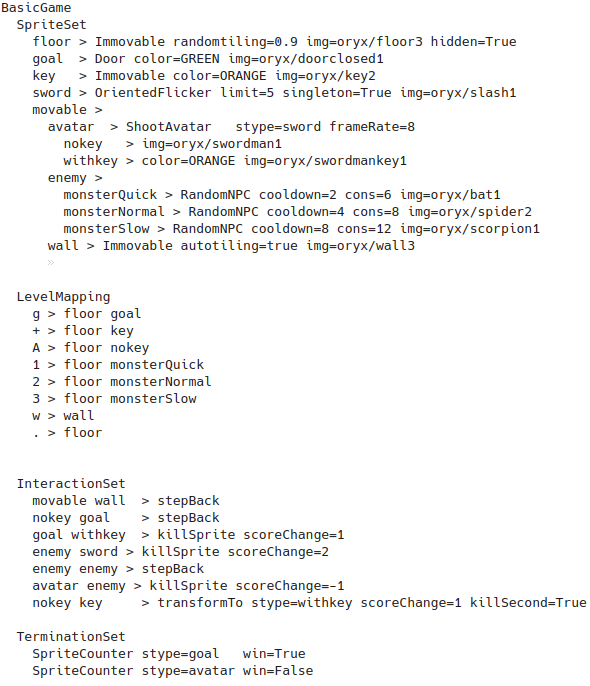
\includegraphics[scale=0.4]{img/presentation/game_def}
            \end{subfigure}
        \end{figure}
    \end{frame}

    %%%%%%%%%%%%%%%%%%%%%%%%%%%%%%%%%%%%%%%%%%%%%%%%%%%%%%%%%%%%%%%%%%%%%%%%%%%%%%%%
    \section{Plan de trabajo}

    \begin{frame}{Metodología}
        \begin{itemize}
            \item Metodología de trabajo basada en \textbf{Scrum}.
            \item Reuniones cada 1-2 semanas:
                \begin{itemize}
                    \item Revisión de objetivos alcanzados.
                    \item Resolución de problemas surgidos.
                    \item Propuesta de nuevos objetivos.
                \end{itemize}
        \end{itemize}
    \end{frame}

    \begin{frame}{Temporización}
        \begin{figure}
            \centering
            \scalebox{0.36}{
                \begin{ganttchart}[%Specs
     y unit title=0.5cm,
     y unit chart=0.7cm,
     vgrid,hgrid,
     title height=1,
     title label font=\bfseries\footnotesize,
     bar/.style={fill=blue},
     bar height=0.4,
     group right shift=0,
     group top shift=0.7,
     group height=.3,
     group peaks width={0.2},
     inline]{1}{36}
    %labels
    \gantttitle{Jul}{3}
    \gantttitle{Ago}{3}
    \gantttitle{Sep}{3}
    \gantttitle{Oct}{3}
    \gantttitle{Nov}{3}
    \gantttitle{Dic}{3}
    \gantttitle{Ene}{3}
    \gantttitle{Feb}{3}
    \gantttitle{Mar}{3}
    \gantttitle{Abr}{3}
    \gantttitle{May}{3}
    \gantttitle{Jun}{3}\\
    % Setting group if any
    \ganttgroup[inline=false]{Estudio}{1}{35}\\
    \ganttbar[inline=false, bar/.style={fill=red}]{Planificación}{1}{4}\\
    \ganttbar[inline=false, bar/.style={fill=red}]{Arquitecturas de planificación}{15}{15}\\
    \ganttbar[inline=false, bar/.style={fill=red}]{Bibliografía complementaria}{34}{35}\\
    
    \ganttgroup[inline=false]{Diseño}{2}{30}\\
    \ganttbar[inline=false, bar/.style={fill=yellow}]{Definición dominio PDDL inicial}{2}{3}\\
    \ganttbar[inline=false, bar/.style={fill=yellow}]{Almacenamiento y gestión de objetivos}{15}{17}
    \ganttbar[inline=false, bar/.style={fill=yellow}]{}{21}{21}\\
    \ganttbar[inline=false, bar/.style={fill=yellow}]{Arquitectura del agente}{21}{22}\\
    \ganttbar[inline=false, bar/.style={fill=yellow}]{Archivo de configuración del sistema}{24}{26}\\
    \ganttbar[inline=false, bar/.style={fill=yellow}]{Definición dominios PDDL nuevos juegos}{27}{28}\\
    \ganttbar[inline=false, bar/.style={fill=yellow}]{Funcionalidad del modo depuración}{29}{30}\\
    
    \ganttgroup[inline=false]{Implementación}{1}{32}\\
    \ganttbar[inline=false, bar/.style={fill=cyan}]{Integración de planificador en GVGAI}{1}{3}\\
    \ganttbar[inline=false, bar/.style={fill=cyan}]{Traducción automática de estados del juego}{5}{12}\\
    \ganttbar[inline=false, bar/.style={fill=cyan}]{Gestión de objetivos}{16}{17}
    \ganttbar[inline=false, bar/.style={fill=cyan}]{}{21}{23}\\
    \ganttbar[inline=false, bar/.style={fill=cyan}]{Control de discrepancias}{21}{23}\\
    \ganttbar[inline=false, bar/.style={fill=cyan}]{Generación automática de archivos de configuración}{26}{27}\\
    \ganttbar[inline=false, bar/.style={fill=cyan}]{Modo depuración}{30}{32}\\
    
    \ganttgroup[inline=false]{Validación}{33}{33}\\
    \ganttbar[inline=false, bar/.style={fill=green}]{Creación de tests}{33}{33}\\
    
    \ganttgroup[inline=false]{Experimentación}{29}{35}\\
    \ganttbar[inline=false, bar/.style={fill=pink}]{Estudio del control de discrepancias}{29}{30}\\
    \ganttbar[inline=false, bar/.style={fill=pink}]{Estudio de la generación de problemas}{35}{35}\\
    
    \ganttgroup[inline=false]{Documentación}{22}{36} \\
    \ganttbar[inline=false, bar/.style={fill=orange}]{Código fuente}{22}{33}\\
    \ganttbar[inline=false, bar/.style={fill=orange}]{Memoria}{34}{36}
\end{ganttchart}

            }
        \end{figure}
    \end{frame}

    %%%%%%%%%%%%%%%%%%%%%%%%%%%%%%%%%%%%%%%%%%%%%%%%%%%%%%%%%%%%%%%%%%%%%%%%%%%%%%%%
    \section{Arquitectura general del sistema}

    \begin{frame}{Objetivo del sistema}
        Dados:

        \begin{enumerate}
            \item Un juego de GVGAI.
            \item Un nivel de ese juego.
            \item Dominio de planificación PDDL que representa el juego.
            \item Archivo de configuración del sistema.
        \end{enumerate}

        El sistema debe resolver el nivel dado, generando para ello los problemas PDDL
        hasta los objetivos especificados \alert{de forma automática} a partir de los estados de
        observación del juego.
    \end{frame}

    \begin{frame}{Arquitectura general}
        \begin{figure}
            \centering
            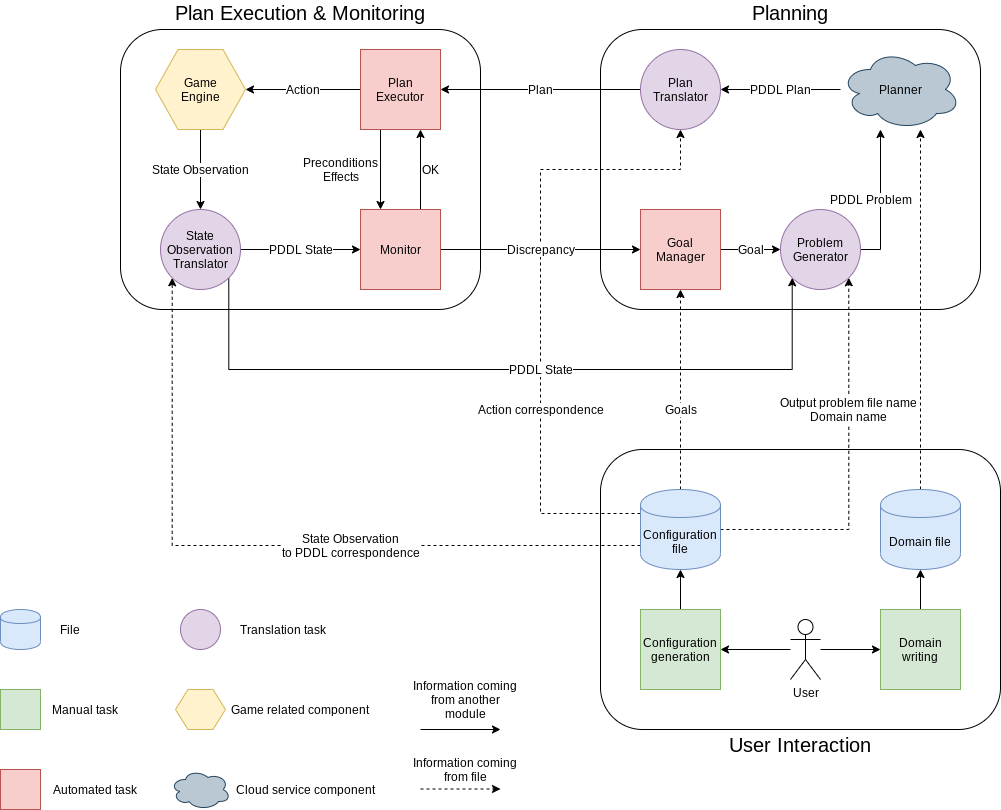
\includegraphics[scale=0.25]{img/presentation/system_arch}
        \end{figure}
    \end{frame}

    %%%%%%%%%%%%%%%%%%%%%%%%%%%%%%%%%%%%%%%%%%%%%%%%%%%%%%%%%%%%%%%%%%%%%%%%%%%%%%%%
    \section{Módulo de planificación}

    %%%%%%%%%%%%%%%%%%%%%%%%%%%%%%%%%%%%%%%%%%%%%%%%%%%%%%%%%%%%%%%%%%%%%%%%%%%%%%%%
    \section{Módulo de ejecución y monitorización}

    %%%%%%%%%%%%%%%%%%%%%%%%%%%%%%%%%%%%%%%%%%%%%%%%%%%%%%%%%%%%%%%%%%%%%%%%%%%%%%%%
    \section{Módulo de interacción con el usuario}

    %%%%%%%%%%%%%%%%%%%%%%%%%%%%%%%%%%%%%%%%%%%%%%%%%%%%%%%%%%%%%%%%%%%%%%%%%%%%%%%%
    \section{Implementación}

    \begin{frame}{Tecnologías utilizadas}
        \begin{figure}
            \centering
            \begin{subfigure}[t]{0.33\textwidth}
                \centering
                
\includegraphics[scale=1]{img/presentation/java}
            \end{subfigure}%
            \begin{subfigure}[t]{0.33\textwidth}
                \centering
                
\includegraphics[scale=0.05]{img/presentation/maven}
            \end{subfigure}%
            \begin{subfigure}[t]{0.33\textwidth}
                \centering
                
\includegraphics[scale=0.03]{img/presentation/python}
            \end{subfigure}
            \par\bigskip
            \begin{subfigure}[t]{0.33\textwidth}
                \centering
                
\includegraphics[scale=0.3]{img/presentation/github}
            \end{subfigure}%
            \begin{subfigure}[t]{0.33\textwidth}
                \centering
                
\includegraphics[scale=1]{img/presentation/github-actions}
            \end{subfigure}%
            \begin{subfigure}[t]{0.33\textwidth}
                \centering
                
\includegraphics[scale=0.15]{img/presentation/travisci}
            \end{subfigure}
        \end{figure}
    \end{frame}

    %%%%%%%%%%%%%%%%%%%%%%%%%%%%%%%%%%%%%%%%%%%%%%%%%%%%%%%%%%%%%%%%%%%%%%%%%%%%%%%%
    \section{Experimentación}

    %%%%%%%%%%%%%%%%%%%%%%%%%%%%%%%%%%%%%%%%%%%%%%%%%%%%%%%%%%%%%%%%%%%%%%%%%%%%%%%%
    \section{Conclusiones}
\end{document}
